\subsubsection{Integration}

Betrachten wir die schwache Form der Impulsbilanz:

\begin{equation}
\int_{\mathcal{B}} \delta\eb\T  \bm{\sigma} \dV = \int_{\mathcal{B}} \delta \bm{u}\T \rho \bm{b} \dV + \int_{\partial\mathcal{B}} \delta \bm{u}\T  \bm{t} \dA \; .
\end{equation}

Dass die Ableitung der Testfunktion $\delta \bm{u}$ und der Verschiebung $\bm{u}$ berechnet werden muss, wurde bereits im vergangenen Abschnitt erläutert. Zusätzlich muss der Term $\delta\eb\T  \bm{\sigma}$ über das gesamte Volumen des Körpers $\mathcal{B}$ integriert werden. Dabei wird in der Finite-Elemente-Methode die Integration über das Volumen des Körpers $\mathcal{B}$ in eine Summe über die Volumen der Elemente $\mathcal{B}^e$ zerlegt:

\begin{equation}
\int_{\mathcal{B}} \delta\eb\T  \bm{\sigma} \dV = \bigcup_{e=1}^{n_{\text{el}}} \int_{\mathcal{B}^e} \delta\eb\T  \bm{\sigma} \dV_e \; .
\end{equation}

Nun kann die Integration auf Elementebene durchgeführt werden. Diese sind aber in der Regel krummlinig berandet und die Integration über das Volumen eines Elements $\mathcal{B}^e$ ist nicht trivial. Daher wird die Integration über das Volumen des Elements $\mathcal{B}^e$ in eine Integration über das Volumen des Referenzelements $\mathcal{B}_{\square}$ umgewandelt:

\begin{equation}
\int_{\mathcal{B}^e} \delta\eb\T  \bm{\sigma} \dV_e = \int_{\mathcal{B}_{\square}} \delta\eb\T  \bm{\sigma} \left| \bm{J} \right| \dV_{\square} \; .
\end{equation}

Dabei ist $\left| \bm{J} \right|$ die Determinante der Jacobi-Matrix $\bm{J}$, die die Transformation von $\mathcal{B}_{\square}$ nach $\mathcal{B}^e$ beschreibt. Damit können wir die Funktion $\delta\eb\T  \bm{\sigma}$ jetzt über eine sehr einfache Geometrie integrieren. Sowohl der Integrand $\delta\eb\T  \bm{\sigma}$ als auch die Determinante der Jacobi-Matrix $\left| \bm{J} \right|$ sind in der Regel nicht konstant, ja sogar gebrochen rationale Funktionen. Die Integrale können daher nicht analytisch gelöst werden. Die bisherige exakte Transformation des Integrals muss nun durch eine numerische Integration approximiert werden. Die numerischen Integrationsformeln werden im Folgenden auch als \textit{Quadraturformeln} bezeichnet. Allgemein gilt für eine Quadraturformel:

\begin{equation}
\int_{\mathcal{B}_{\square}} f(\bm{\xi}) \dV_{\square} \approx \sum_{i=1}^{n_{\text{qp}}} w_i f(\bm{\xi}_i) \; .
\end{equation}

Die Integration der Funktion $f(\bm{\xi})$ über das Gebiet $\mathcal{B}_{\square}$ wird also ersetzt durch eine Summe über die Funktionswerte $f(\bm{\xi}_i)$ an den Integrationspunkten $\bm{\xi}_i$, multipliziert mit den Gewichten $w_i$. Die Anzahl der Integrationspunkte $n_{\text{qp}}$ hängt von der gewünschten Genauigkeit der Integration ab. Die Integrationspunkte und Gewichte sind für die im vorangegangenen Abschnitt beschriebenen Elemente in Tabellen zusammengestellt. Die Genauigkeit der Integration hängt ma$\beta$geblich von der Form der Funktion $f(\bm{\xi})$ ab. Allgemein gilt, dass die Genauigkeit der Integration mit der Anzahl der Integrationspunkte steigt. Die in den FE-Programmen meist verwendeten Integrationspunkte und Gewichte entsprechen den Gau$\beta$-Quadraturregeln oder sind zumindest an diese angelehnt. Bei der Gau$\beta$-Quadraturregel werden die Integrationspunkte so gewählt, dass die Integration einer Polynomfunktion $f(\bm{\xi})$ bis zu einem bestimmten Grad genau ist. Die Gewichte $w_i$ sind so gewählt, dass die Summe der Gewichte gleich der Fläche des Integrationsgebiets ist. Mit einer Integrationsordnung $m$ kann mit der Gau$\beta$-Quadratur ein Polynom $(2m - 1)$-ten Grades exakt integriert werden. Betrachten wir erneut die schwache Form und schreiben den Integranden $\delta\eb\T  \bm{\sigma}$ als $\delta\eb\T  \bm{\sigma} = \delta\eb\T  \mathbb{C} \eb$, dann sehen wir, dass rechts und links der Materialtangente $\mathbb{C}$ die räumliche Ableitung von $\bm{u}_h$ und $\delta\bm{u}_h$ steht. Wenn wir nun quadratische Formfunktionen verwenden, dann ist die Ableitung der Formfunktionen zumindest in einer Koordinatenrichtung weiterhin quadratisch. Durch die Multiplikation im Integranden müssen wir also ein Polynom 4. Grades integrieren. Nach der obigen Definition ist hierfür eine Quadraturformel 3. Grades erforderlich.

\begin{framed}
\textbf{Notwendige Ordnung der Integration}\\
Für die Integration der Steifigkeitsmatrix der FEM mit Elementen mit Formfunktionen der Ordnung $n$ ist eine Quadraturformel der Ordnung:

\begin{equation*}
m = \frac{n+1}{2}
\end{equation*}
erforderlich.
\end{framed}

Nachfolgende Tabellen zeigen die 1D- und 2D-Quadraturformeln.

\begin{figure}[!htbp]
\centering
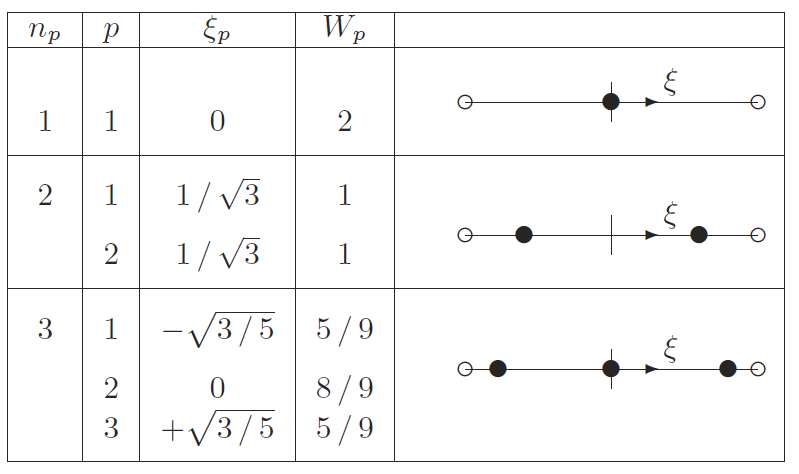
\includegraphics[width=0.625\linewidth]{files/Wriggers_GQ_01-1fe6a7f6344b6ab2a225d181d5bca432.png}
\caption[]{1D-Gau$\beta$-Quadraturformeln für verschiedene Ordnungen $m$ nach \cite{wriggers2008nonlinear}.}
\label{lineQuadrature}
\end{figure}

\begin{figure}[!htbp]
\centering
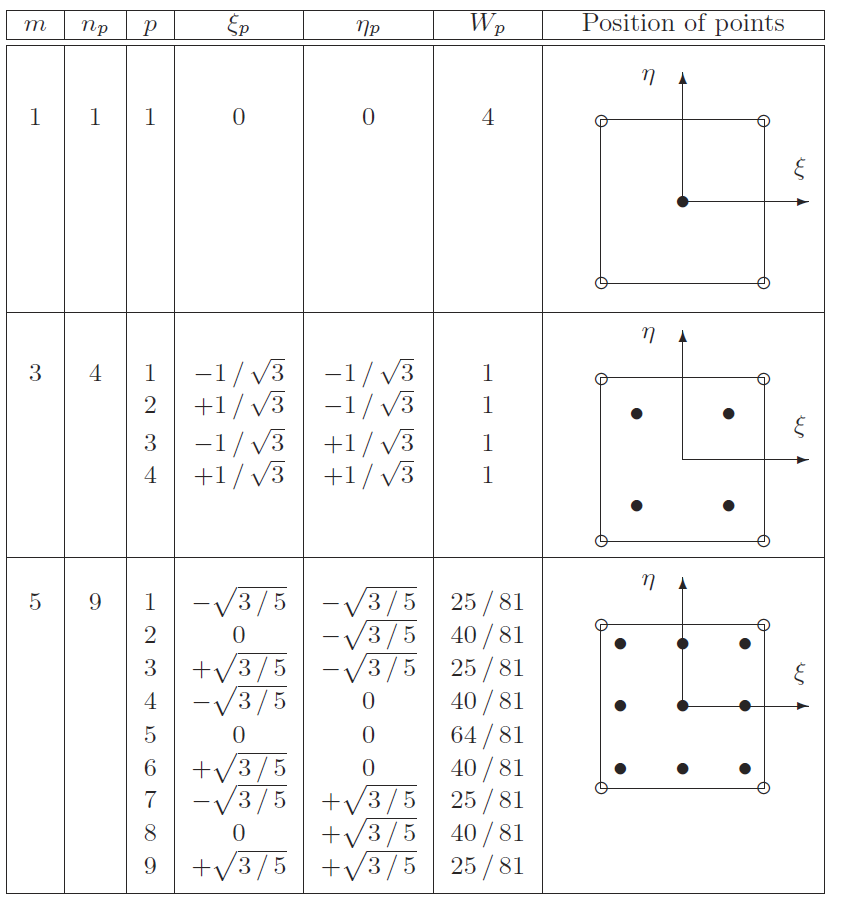
\includegraphics[width=0.625\linewidth]{files/Wriggers_GQ_02-d7a6daa03fb1eafb11f2f6a808c915f2.png}
\caption[]{2D-Gau$\beta$-Quadraturformeln für Rechteckelemente verschiedener Ordnung $m$ nach \cite{wriggers2008nonlinear}.}
\label{squareQuadrature}
\end{figure}

\begin{figure}[!htbp]
\centering
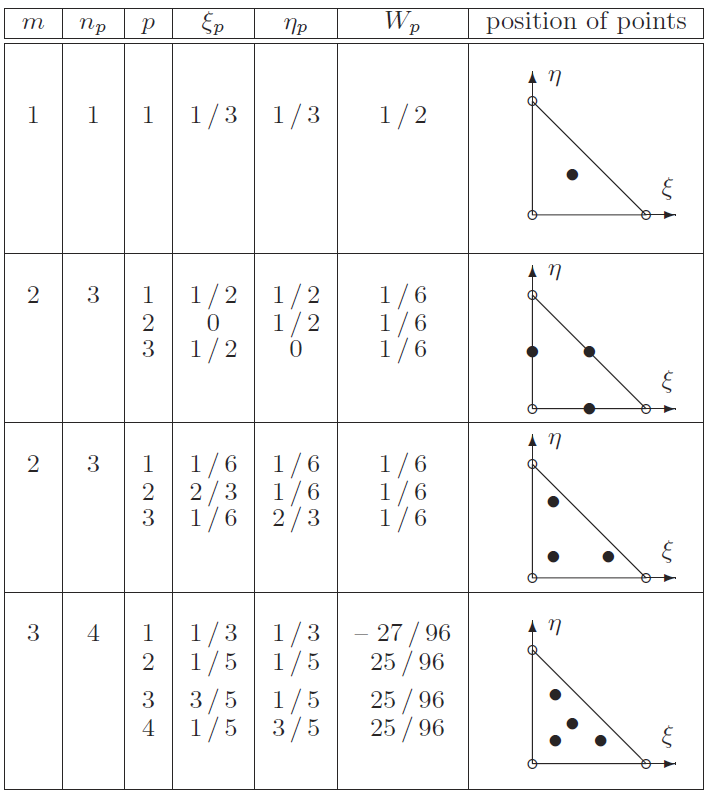
\includegraphics[width=0.625\linewidth]{files/Wriggers_GQ_03-44827e8d787266f893a14150a814a302.png}
\caption[]{2D-Gau$\beta$-Quadraturformeln für Dreieckselemente verschiedener Ordnung $m$ nach \cite{wriggers2008nonlinear}.}
\label{triQuadrature}
\end{figure}

\paragraph{Beispiel: 1D-Integration}

Wir möchten das Polynom $f(x) = \frac{1}{2} x^4 + 6x + 4$ über das Intervall $[ -1,1]$ integrieren. Die exakte Lösung ist:
\begin{equation*}
\int_{-1}^{1} \left(\frac{1}{2} x^4 + 6x + 4\right) \, \mathrm{d}x = \left[\frac{1}{10} x^5+2x^3+4x \right]_{-1}^{1} = 12.2
\end{equation*}

Da wir im Intervall $[ -1,1]$ integrieren, können wir direkt die Gau$\beta$-Quadraturformeln verwenden. Wir müssen nicht die Jacobideterminante berechnen.
Verwenden wir jetzt eine Integrationsordnung mit einem Integrationspunkt, so ergibt sich:
\begin{align*}
\xi_p &= 0  & w_p &= 2 \\
\int_{-1}^{1} f(x) \, \mathrm{d}x &= \sum_{p=1}^{1} w_p f(\xi_p) \\
\int_{-1}^{1} f(x) \, \mathrm{d}x &= 2 \cdot 4  = 8
\end{align*}

Mit dieser Integrationsordnung ergibt sich also ein Fehler von 34 \%.

Als nächstes nehmen wir eine Integrationsordnung mit zwei Integrationspunkten:
\begin{align*}
\xi_p &= \pm \frac{1}{\sqrt{3}} & w_p &= 1 \\
\int_{-1}^{1} f(x) \, \mathrm{d}x &= \sum_{p=1}^{2} w_p f(\xi_p)  \\
\int_{-1}^{1} f(x) \, \mathrm{d}x &= 1 \cdot 6.06  + 1 \cdot 6.06 = 12.111
\end{align*}

Hier ergibt sich nur noch ein Fehler von 1 \%.

Erst eine Integrationsordnung mit drei Integrationspunkten liefert das exakte Ergebnis:
\begin{align*}
\xi_p &= 0, \pm \sqrt{\frac{3}{5}} & w_p &= \frac{8}{9}, \frac{5}{9} \\
\int_{-1}^{1} f(x) \, \mathrm{d}x &= \sum_{p=1}^{3} w_p f(\xi_p) \\
\int_{-1}^{1} f(x) \, \mathrm{d}x &= \frac{5}{9} \cdot 7.78  + \frac{8}{9} \cdot 4 + \frac{5}{9} \cdot 7.78  = 12.2
\end{align*}

\begin{framed}
\textbf{Fragen zum Kapitel}\\
\textbf{Integration}

\begin{itemize}
\item Warum müssen wir die schwache Form der Impulsbilanz numerisch integrieren?
\item Wie lautet die allgemeine Formel für die Quadratur einer Funktion $f(x)$ über ein Referenzgebiet?
\item Wie lässt sich die Genauigkeit der numerischen Integration erhöhen?
\item Welche Aussage ist richtig?\begin{itemize}
\item Eine Erhöhung der Integrationsordnung führt zu einer höheren Genauigkeit.
\item Eine Erhöhung der Integrationsordnung führt zu einer höheren Anzahl an Integrationspunkten.
\item Bei zu wenigen Integrationspunkten verhält sich das Element zu ``weich''.
\item Unzulässige Null-Energiemodi sind ein Indikator für zu wenige Integrationspunkte.
\item Ist die notwendige Anzahl an Integrationspunkten erreicht, führt auch eine Erhöhung der Integrationsordnung nicht zu einer besseren Konvergenz.
\end{itemize}
\end{itemize}
\end{framed}